\documentclass[11pt]{article}
\usepackage[top=2cm,bottom=2cm,left=1.75cm,right= 1.75cm]{geometry}
%\geometry{landscape}                % Activate for for rotated page geometry
\usepackage[parfill]{parskip}    % Activate to begin paragraphs with an empty line rather than an indent
\usepackage{graphicx}
\usepackage{amssymb}
\usepackage{epstopdf}
\usepackage{amsmath}
\usepackage{multirow}
\usepackage{hyperref}
%\usepackage{changepage}
\usepackage{lscape}
%\usepackage{ulem}
\usepackage{multicol}
\usepackage{setspace}
\usepackage{dashrule}
\usepackage[usenames,dvipsnames]{color}
\usepackage{enumerate}
\usepackage{enumitem}
\usepackage{float}
\newcommand{\urlwofont}[1]{\urlstyle{same}\url{#1}}
\newcommand{\degree}{\ensuremath{^\circ}}
\newcommand{\hl}[1]{\textbf{\underline{#1}}}
\newcommand\given[1][]{\:#1\vert\:}

% footnote citation
\usepackage[style=authortitle-ibid, maxnames=3,natbib=true,sortcites=true,block=space]{biblatex}
\bibliography{final}

% color hyperlinks
%\usepackage[colorlinks=false,pdfborder={0 0 0},urlcolor= MidnightBlue,colorlinks=true,linkcolor= MidnightBlue, citecolor= MidnightBlue,backref=true]{hyperref}

\DeclareGraphicsRule{.tif}{png}{.png}{`convert #1 `dirname #1`/`basename #1 .tif`.png}

\newenvironment{choices}{
\begin{enumerate}[(a)]
}{\end{enumerate}}

%\newcommand{\soln}[2]{\textcolor{MidnightBlue}{\textit{#2}}}{} 		% solutions
\newcommand{\soln}[2]{\vspace{#1}}{}						% exam, handout, etc.

%\newcommand{\solnMult}[1]{\textbf{\textcolor{MidnightBlue}{\textit{#1}}}}	% uncomment for solutions
\newcommand{\solnMult}[1]{ #1 }	% uncomment for handouts

%\newcommand{\tf}[1]{ \textbf{\textcolor{MidnightBlue}{\textit{#1}}} }	% uncomment for solutions
\newcommand{\tf}[1]{}	% uncomment for handouts

%\newcommand{\pts}[1]{ \textbf{{\small \textcolor{BurntOrange}{(#1)}}} }	% uncomment for solutions
\newcommand{\pts}[1]{ \textbf{{\small \textcolor{black}{(#1)}}} }	% uncomment for handouts

\newcommand{\note}[1]{ \textbf{\textcolor{red}{[#1]}} }	% uncomment for handouts

\newcommand{\qt}[1]{\textcolor{RoyalBlue}{\textbf{\textit{#1.}}}}

\renewcommand{\emph}[1]{\underline{\textbf{#1}}}

\newcommand{\reference}[1]{ \textbf{\textcolor{red}{[#1]}} }

%\newcommand{\fb}[3]{
%  \textcolor{NavyBlue}{\textbf{Question Feedback:} #1} \\$\:$\\
%  \textcolor{NavyBlue}{\textbf{This question refers to the following learning objective(s):}\\
%  \textbf{\textit{#2:}} #3}
%}


\begin{document}

\begin{titlepage}

\enlargethispage{\baselineskip}


STA 214 \hfill Dr. Evans \\
Fall 2022	\hfill Exam 1\\

\vspace{-2cm}

\begin{center}
{\Huge Exam 1}	
\end{center}

$\:$ \\

\textbf{Last Name:} \rule{5cm}{0.5pt}	\hfill	 \textbf{First Name:}  \rule{5cm}{0.5pt}	 \\
$\:$ \\
%\textbf{Section:} A (11 AM) $\quad$ B (9:30 AM) \hfill	
%\textbf{Team Name:}  \rule{7cm}{0.5pt} \\
$\:$ \\

\textit{I hereby state that I have not communicated with or gained information in any way from other students or any outside resource during this exam. I agree to abide by the rules stated below, and to abide by the Wake Forest Honor Code. All work is my own. I understand that any violation of this agreement will be reported to the Honor Council and will result, at minimum, in a 0 on this exam.}
\[ Signature: \rule{7cm}{0.5pt}\]

\hdashrule[0.5ex]{\textwidth}{0.5pt}{3mm}

\textbf{All work on this exam must be your own.}

{\small
\begin{enumerate}
\item You have 50 minutes to complete the exam.
\item Show all your work on the open ended questions in order to get partial credit. No credit will be given for open ended questions where no work is shown, even if the answer is correct.
\item You are allowed a calculator, however you may not share a calculator with another student during the exam. The calculator must be only a calculator, and may not be connected to the internet. 
\item You are allowed to ask clarification questions to me, but you may not ask anyone else. 
\item You are \hl{not} allowed a cell phone, even if you intend to use it as a calculator or for checking the time. You are \hl{not} allowed a music device or headphones, notes, books, or other resources. 
\item You may \hl{not} communicate with anyone other than myself during the exam.
\item Write clearly and be clear. Make it easy to find your answers. 
\end{enumerate}
}
\begin{center}
{\Large Good luck!}
\end{center}
\hdashrule[0.5ex]{\textwidth}{0.5pt}{3mm}

%\begin{center}
%\includegraphics[width=0.5\textwidth]{../figures/bubbles_new}
%\end{center}



\end{titlepage}

\pagebreak

%%%%%%%%%%%%%%%%%%%%%%%%%%%%%%%%%%%%%%%
$\:$ \\
\thispagestyle{empty}
\pagebreak

%%%%%%%%%%%%%%%%%%%%%%%%%%%%%%%%%%%%%%%
\setcounter{page}{1}
%%%%%%%%%%%%%%%%%%%%%%%%%%%%%%%%%%%%%%%

%\rule{\textwidth}{1pt}
%\begin{center}
%\textit{Answer questions \ref{DriveStart} to \ref{DriveEnd} based on the information %below.} \\
%\end{center}
\rule{\textwidth}{0.5pt}

\textbf{The Data} 

You are contacted by the US Small Business Administration (SBA), a government agency dedicated to helping support small businesses. The SBA provides loans to small businesses, but some businesses \textit{default} on their loan (i.e., fail to pay it back). Researchers at the SBA are interested in predicting whether a business will default on the loan, and they have collected a random sample of 998 different loans. For each loan, we have the following variables:

\begin{itemize}
\item \textit{Default}: Whether the business defaulted (0 = no, 1 = yes)
\item \textit{Amount}: The amount (in US dollars) of the original loan
\item \textit{NewBusiness}: Whether the business receiving the loan is a new business (1) or an existing business (0)
\end{itemize}

\textbf{Research question:} Researchers at the SBA want you to investigate the following question: \textit{Is there a relationship between loan amount and whether a business defaults on the loan, after accounting for the age of the business (whether it is new or not).}

\rule{\textwidth}{1pt}

\begin{enumerate}

\item (3 pts) We will begin by investigating the relationship between loan amount and loan default (we will add NewBusiness to the model later). Choose \textit{one} of the following population models for the relationship between loan amount and loan default, and explain your choice. (Let $Y_i$ denote whether the business defaulted on the loan, and assume that the shape/linearity assumption is satisfied).

\begin{enumerate}
\item $Y_i = \beta_0 + \beta_1 \ Amount_i + \varepsilon_i$
\item $Y_i \sim N(\pi_i, \sigma^2) \hspace{1cm} \pi_i = \beta_0 + \beta_1 \ Amount_i$
\item $Y_i \sim Bernoulli(\pi_i) \hspace{1cm} \log \left( \dfrac{\pi_i}{1 - \pi_i} \right) = \beta_0 + \beta_1 \ Amount_i + \varepsilon_i$
\item $Y_i \sim Bernoulli(\pi_i) \hspace{1cm} \log \left( \dfrac{\pi_i}{1 - \pi_i} \right) = \beta_0 + \beta_1 \ Amount_i$
\item $Y_i \sim Bernoulli(\pi_i) \hspace{1cm} \pi_i = \beta_0 + \beta_1 \ Amount_i$
\end{enumerate}



\newpage


We fit the model from Question 1, and obtain the following output:

\textbf{Model 1:}

\begin{verbatim}
              Estimate Std. Error 
(Intercept) -1.160e-01  2.558e-01
Amount      -5.713e-06  1.010e-06 
---

    Null deviance: 923.58  on 997  degrees of freedom
Residual deviance: 889.82  on 996  degrees of freedom
\end{verbatim}

\rule{\textwidth}{1pt}

\item (3 pts) Based on the output above, write down the equation of the fitted model.

\vspace{3cm}

\item (3 pts) Interpret the slope of the fitted model in terms of the odds.

\vspace{3cm}

\item (3 pts) What is the predicted probability that a business will default on a loan of \$200,000?


\newpage

To answer the research question, we need to include the NewBusiness variable to the model. Below is an empirical log odds plot showing the relationship between loan amount and whether the business defaulted, with a separate line fit for new and existing businesses.

\begin{center}
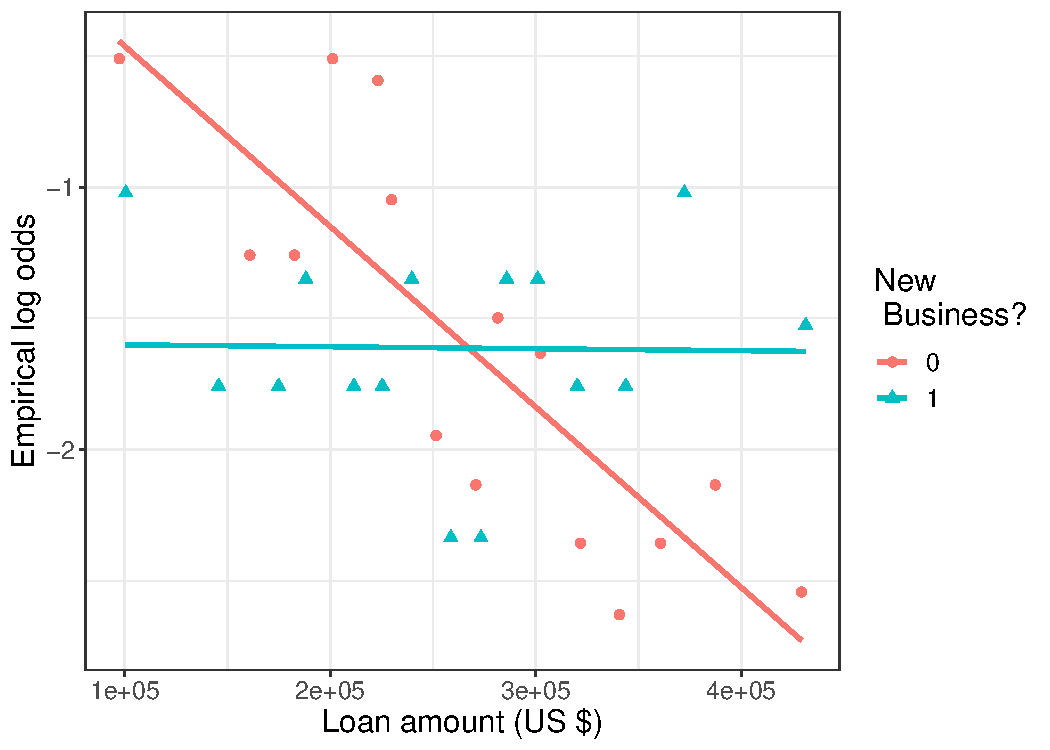
\includegraphics[scale=0.7]{empirical_log_odds_exam_1.pdf}
\end{center}

\rule{\textwidth}{1pt}


\item (4 pts) Using the empirical log odds plot, write down a population model that allows us to investigate the research question. Use appropriate notation, and explain your reasoning for choosing the model.

\pagebreak

You fit the model from Question 5, and two other models as well. The output for these three models is shown below, in no particular order:\\


\textbf{Model 2:}

\begin{verbatim}
glm(formula = Default ~ NewBusiness, family = binomial, data = sba_data)

            Estimate Std. Error 
(Intercept) -1.50729    0.09408 
NewBusiness -0.21249    0.20397 
---

    Null deviance: 923.58  on 997  degrees of freedom
Residual deviance: 922.46  on 996  degrees of freedom
\end{verbatim}

\vspace{2cm}

\textbf{Model 3:} 

\begin{verbatim}
glm(formula = Default ~ Amount + NewBusiness, family = binomial, 
    data = sba_data)
    
              Estimate Std. Error 
(Intercept) -3.026e-02  2.630e-01 
Amount      -5.796e-06  1.012e-06  
NewBusiness -2.870e-01  2.076e-01 
---

    Null deviance: 923.58  on 997  degrees of freedom
Residual deviance: 887.84  on 995  degrees of freedom
\end{verbatim}

\vspace{2cm}

\textbf{Model 4:}

\begin{verbatim}
glm(formula = Default ~ Amount * NewBusiness, family = binomial, 
    data = sba_data)

                     Estimate Std. Error 
(Intercept)         3.257e-01  2.918e-01 
Amount             -7.286e-06  1.166e-06 
NewBusiness        -1.963e+00  6.443e-01 
Amount:NewBusiness  6.961e-06  2.440e-06 
---

    Null deviance: 923.58  on 997  degrees of freedom
Residual deviance: 879.84  on 994  degrees of freedom
\end{verbatim}


\pagebreak

\rule{\textwidth}{1pt}

\item (4 pts) The SBA wants to identify loans for which the predicted probability of default is at least 0.3. For \textit{existing} businesses, which loan amounts correspond to a predicted probability of at least 0.3? Use the fitted model corresponding to your population model from Question 5.

\vspace{5cm}

\item (3 pts) Now let's address the original research question. We want to test whether there is a relationship between loan amount and whether a business defaults on the loan, after accounting for whether the business is new. Using your model from Question 5, write down null and alternative hypotheses, in terms of one or more model parameters, for this research question.

\vspace{5cm}

\item (3 pts) Which test (Wald, Likelihood ratio, or both) could you use to test your hypotheses from Question 7? Explain your answer.

\pagebreak


\item (4 pts) Using the output from Model 1 and/or Model 2 and/or Model 3 and/or Model 4, calculate a test statistic for your hypotheses in Question 7. What distribution will you compare your test statistic with to calculate a p-value (give the name and degrees of freedom, if applicable, for the distribution)?


\pagebreak


%%%%%%%%%%%%%%%%%%%%%%%%%%%

\textbf{Part II: Maximum likelihood estimation}

\textit{(This question is unrelated to the SBA data or the previous questions)}

Suppose we are told that we have a certain random variable $Y$, which can take three possible values: $Y = -1$, 0, or 1. We are told that the probability for each outcome is
\begin{itemize}
\item $P(Y = 0) = \pi_0$
\item $P(Y = -1) = 5 \pi_0$
\item $P(Y = 1) = 1 - 6 \pi_0$
\end{itemize}
where the parameter $\pi_0$ is unknown. We observe data $-1, 0, 0, 1, 1, -1, 0$, and we want to estimate $\pi_0$ from the data.

\rule{\textwidth}{1pt}


\item (6 pts) Using the method of maximum likelihood, solve for the maximum likelihood estimate of $\pi_0$. Show your work.  

\pagebreak

%%%%%%%%%%%%%%%%%%%%%%%%%%%%%%%%%%%%%%%%


\huge{You are done!!! Whooo!!!}


%%%%%%%%%%%%%%%%%%%%%%%%%%%%%%%%%%%%%%%%


\end{enumerate}

%%%%%%%%%%%%%%%%%%%%%%%%%%%%

%\pagebreak

%\hdashrule[0.5ex]{\textwidth}{0.5pt}{3mm}
%\begin{center}
%\renewcommand{\arraystretch}{1.5}
%\begin{tabular}{| l | c | c | c | c | c | c  || c |}
%\hline
%				& 		& 		& 		& 		&	&  	&\\
%				& Q1-Q3		& Q4-6		& Q7		& Q8-Q10		 & Q11-Q12	 & Q13 & Total	\\
%\hline
%Points earned		& \textcolor{white}{xxxxx} &	\textcolor{white}{xxxxx}	& \textcolor{white}{xxxxx}	&	\textcolor{white}{xxxxx}&%\textcolor{white}{xxxxx}	&	\textcolor{white}{xxxxx} &	\textcolor{white}{xxxxx} \\
%\hline
%Available points	& 9 		& 12		& 9		& 9		&7 & 4 					& 50 \\
%\hline
%\end{tabular}

%\end{center}

\end{document}
